
% !TEX TS-program = xelatex
% !TEX encoding = UTF-8 Unicode

% \documentclass[AutoFakeBold]{LZUThesis}
\documentclass[]{LZUThesis}
\usepackage{hyperref}
\usepackage{multirow}
\usepackage[numbers,sort&compress]{natbib}
\newcommand{\upcite}[1]{\textsuperscript{\textsuperscript{\cite{#1}}}}

\begin{document}

\title{{粗糙链孢菌顺序四分子分析}}

\entitle{{Sequential tetramolecule analysis of \textit{Neurospora crassa}}}

\author{生物信息学班 李泽华 320210928501}
\major{遗传学}
\advisor{王铭裕}
\college{生命科学学院}
\grade{2021级}


\frontmatter

\ZhAbstract{
本研究聚焦于粗糙链孢霉(\textit{Neurospora crassa})的遗传特性,该真菌具有一系列便于遗传分析的特点,包括单倍体子囊孢子、快速繁殖等。该研究旨在通过顺序四分子的遗传学分析方法,深入理解粗糙链孢霉基因的分离和连锁交换规律。

研究目的与方法部分明确了研究的目标,包括了解粗糙链孢霉的生活史和特性,掌握顺序四分子的遗传学分析方法,并通过着丝粒作图深入理解基因的分离和连锁交换定律。详细介绍了实验所使用的材料、试剂和器具,以及实验步骤,包括菌种活化、杂交、显微镜观察等。

实验结果与分析部分呈现了观察到的子囊类型及其排列方式,以及各组员的观察数据。此外,还发现了一些异常类型的子囊孢子,通过对这些异常的解释,提高了对实验结果的理解。最后,进行了数据分析,计算了重组率,并通过换算得到基因与着丝粒的距离。

综合而言,该研究在深入理解粗糙链孢霉遗传学特性的基础上,通过实验得到了详实的结果,并通过数据分析得出了有意义的结论,为后续的遗传学研究提供了重要参考。
}{粗糙链孢霉,
遗传特性,
顺序四分子,
遗传学分析,
子囊孢子,
连锁交换,
着丝粒,
重组率,
基因分离}

\EnAbstract{
This study focuses on the genetic characteristics of Neurospora crassa, a filamentous fungus with features conducive to genetic analysis, such as haploid ascospores and rapid reproduction. The research aims to deepen the understanding of the segregation and linkage patterns of Neurospora crassa genes using a genetic analysis approach called tetrad analysis.

The objectives and methods of the study clearly outline its goals, including understanding the life history and characteristics of Neurospora crassa, mastering the genetic analysis method of tetrad analysis, and gaining a comprehensive understanding of gene segregation and linkage exchange laws through centromere mapping. The materials, reagents, and equipment used in the experiment, as well as the experimental procedures, including strain activation, hybridization, and microscopic observation, are detailed.

The results and analysis section presents the observed types and arrangements of ascospores, along with the observation data from each group member. Additionally, some abnormal types of ascospores were identified, and their anomalies were explained, enhancing the understanding of the experimental results. Finally, data analysis was conducted, recombination rates were calculated, and gene-to-centromere distances were determined through conversion.

In summary, this study, building upon a deep understanding of the genetic characteristics of Neurospora crassa, provides detailed results through experimentation and meaningful conclusions through data analysis. It serves as a significant reference for subsequent genetic research.
}{Neurospora crassam,
Genetic characteristics,
Tetrad analysis,
Genetic analysis,
Ascospores,
Linkage exchange,
Centromere,
Recombination rate,
Gene segregation}

\customcontent

\mainmatter

\chapter{\texorpdfstring{绪 \quad 论}{绪论}}
粗糙链孢霉(Neurospora crassa)是一种广泛应用于真菌遗传学研究的模式生物,其单倍体子囊孢子和快速的繁殖特性使其成为理想的实验材料。本研究旨在通过对粗糙链孢霉遗传特性的深入分析,探讨该真菌基因的分离和连锁交换规律,以期为更广泛的遗传学研究提供有益的参考。

首先,了解粗糙链孢霉的生活史和特性对于深入研究其遗传学至关重要。本研究将通过详细描述这些特性,为后续实验设计提供基础。

其次,顺序四分子是一种常用于真菌遗传学研究的方法,通过此方法可以深入了解基因的分离和连锁交换规律。本研究将应用顺序四分子的遗传学分析方法,以揭示粗糙链孢霉基因的遗传机制。

在实验方面,通过使用特定的材料、试剂和器具,以及详细规划的实验步骤,本研究将从菌种活化到显微镜观察,系统地展示实验的操作过程,确保研究的可重复性和可靠性。

最后,通过实验结果的观察和数据分析,我们将能够得出关于粗糙链孢霉遗传特性的深刻结论,为进一步的遗传学研究提供实质性的支持。

\chapter{研究背景}
\section{粗糙链孢菌的特性}
粗糙链孢霉(\textit{Neurospora crassa})又称红色面包霉, 属于真菌中的子囊菌纲, 球壳目, 脉孢菌属, 目前已知4\~5种.
粗糙脉孢霉是低等的真核生物, 对于其进行遗传分析具有以下特点:\par
1. 子囊孢子是单倍体,没有显隐性,其表型直接反应其基因型;\par
2. 一次只分析一个减数分裂的产物,就可观察到遗传结果,简单易行;\par
3. 体积小,易培养,繁殖快,一次杂交就能产生大量的后代,便于获得正确的统计学结果;\par
4. 既能进行有性生殖,又能进行无性生殖,其染色体的结构和功能类似于高等动植物,研究结果可在遗传学广泛应用;\par
5. 子囊孢子在子囊中的线性排列顺序,与减数分裂中期染色体在赤道板两侧的排列顺序相同,便于观察。\par
因此,粗糙链孢霉是进行基因分离和连锁交换遗传分析的好材料。

\section{粗糙链孢菌的生活史}
粗糙链孢菌的生活史如图\ref{fig:1}所示。\par
\begin{figure}[htbp]
    \centering
    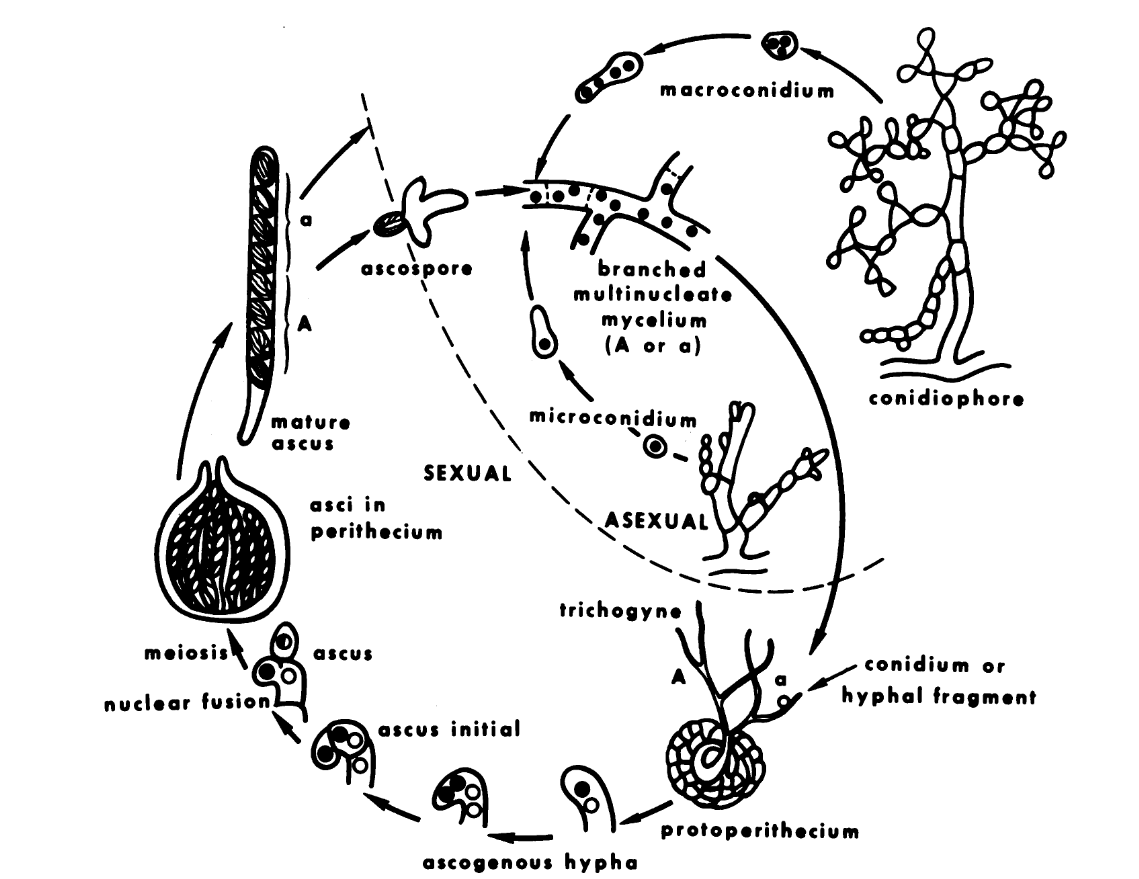
\includegraphics[width=0.7\textwidth]{img/lifecircle.png}
    \caption{life cycle of \textit{Neurospora crassa}引用自\upcite{doi:10.1128/jb.113.2.1015-1025.1973}}
    \label{fig:1}
\end{figure}
单倍体菌丝体通过两个过程进行无性繁殖:(1)现有菌丝体的简单增殖,以及(2)形成分生孢子(宏观和微观),分生孢子可以分散,然后发芽产生新的菌丝体。在有性周期中,交配只能发生在不同交配类型A和a的个体品系之间。受精是通过一种交配类型的分生孢子或菌丝体的细胞核通过毛线虫进入相反交配类型的原上皮壳而发生的。相反交配类型的核在原白囊内发生融合,形成合子 (2N) 核。

\section{顺序四分子(ordered tetrad)}
真菌的子囊类型依据内部子囊孢子排列的特点可进一步区分为顺序四分子(ordered tetrad)
和非顺序四分子(unordered tetrad)。顺序四分子因其所在子囊狭小,限制了减数分裂后期
两个子细胞核的自由移动,造成子细胞在子囊内的随机分布与分裂后期纺锤体的方向直接相牵,
如果某基因与着丝点间发生交换,则可以通过子囊孢子在子囊中的排列情况加以研究,进而计算出该
基因与着丝点间的遗传距离,这就是顺序四分子的着丝粒作图(centromere mapping)。
顺序四分子分析通常以粗链孢菌(Neurospora crassa)为代表\upcite{YCZZ201911008}。正如戴灼华和王亚馥主编的教材中
总结的那样,顺序四分子在遗传分析中具有独特的优越性,可以揭示其他遗传分析方法所不能发现的遗传
本质\upcite{dai2016}。教材具体总结了顺序四分子分析的4个优点:\par
\begin{enumerate}
    \item 将着丝粒视作一个基因座,计算某一基因与着丝粒的重组率;\par
    \item 子囊孢子的对称性,证明了减数分裂是一个交互的过程;\par
    \item 可检验染色体单体的交换是否存在干涉现象,并且可以利用它来研究基因转变现象;\par
    \item 发现双交换不仅可以包括4线中的2线,而且还可以包括3线或4线。\par
\end{enumerate}
由此可计算出某一基因与着丝粒的重组率,即着丝粒作图(centromere mapping)。
\begin{equation}\label{eq:1}
Recombination~Values = \frac{ascospores~in~the~second~division}
{total~number~of~ascospores}\times \frac{1}{2}\times 100\%
\end{equation}
\begin{figure}[htbp]
    \centering
    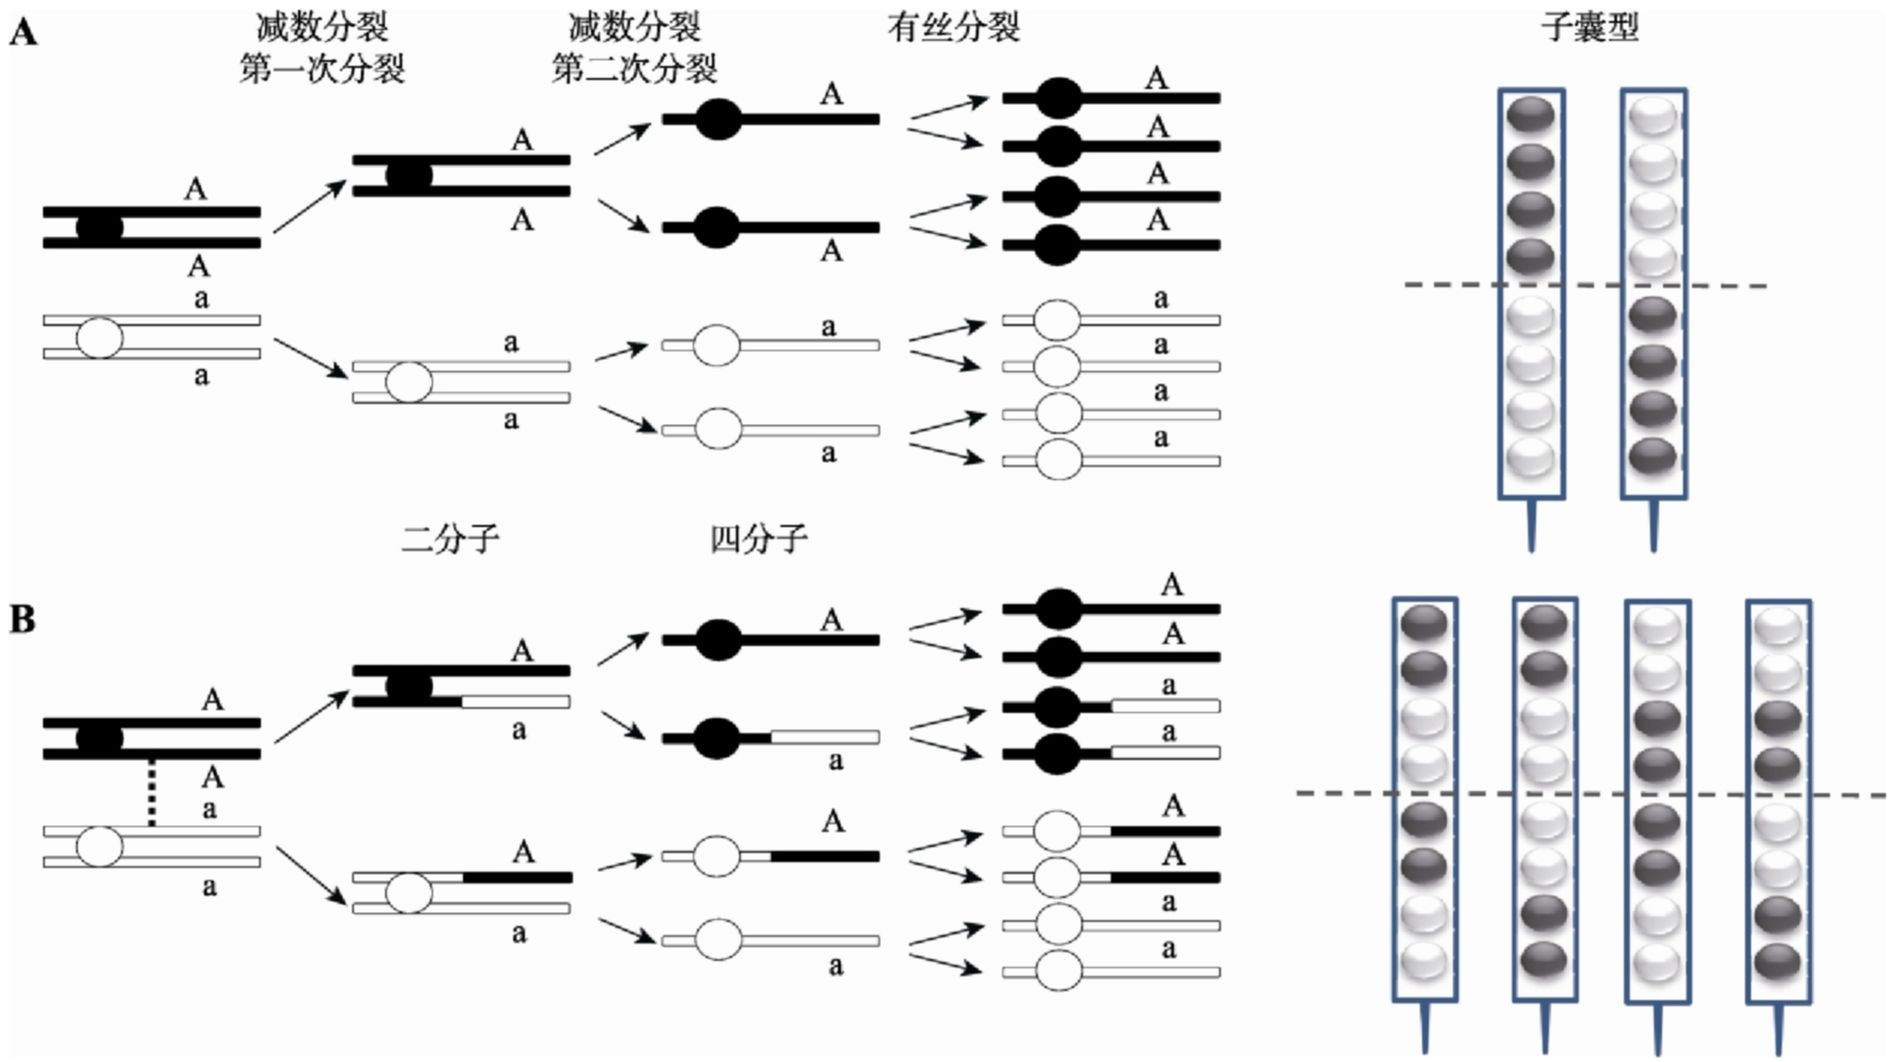
\includegraphics[width=0.6\textwidth]{img/7orderedtetrad}
    \caption{Six classes of tetrad in centromere mapping引用自\upcite{YCZZ201911008}}
    \label{fig:2}
\end{figure}

\chapter{研究目的与方法}
\section{研究目的}
\begin{itemize}
    \item 了解粗糙链孢霉的生活史及其特性
    \item 了解对粗糙链孢霉杂交后代的表型分析, 掌握顺序四分子的遗传学分析方法
    \item 通过有关基因的着丝粒作图, 进一步理解基因的分离和连锁交换定律
\end{itemize}

\section{研究方法}
\subsection{实验材料与数据收集}
\begin{itemize}
    \item 实验材料: 粗糙链孢霉
    \begin{itemize}
        \item 野生型菌株($Lys^+,mt^+$)
        \item 赖氨酸缺陷型菌株($Lys^-,mt^-$)\par
        本实验使用的子囊孢子由两者杂交而来. 黑色孢子为野生型, 而赖氨酸缺陷型孢子成熟迟, 在野生型孢子变黑后仍未变黑, 而呈现棕色.
    \end{itemize}
    \item 实验试剂:
    \begin{enumerate}
        \item 5\%NaClO溶液
        \item 5\%苯酚溶液
        \item 马铃薯培养基
        \item 补充培养基(每升马铃薯培养基中加入0.1g赖氨酸)
        \item 玉米杂交培养基
    \end{enumerate}
    \item 实验器具:\par
    超净工作台, 恒温培养箱, 显微镜, 解剖镜, 高压灭菌锅, \ldots
    \item 数据收集: \par
    通过显微镜观察子囊果中的子囊孢子排列情况, 统计各类子囊孢子的数量
\end{itemize}

\subsection{实验步骤}
\begin{enumerate}
    \item 菌种活化\par
    将粗糙链孢霉野生型和赖氨酸缺陷型菌种从冰箱中取出,
    在超净工作台上分别接种到两支马铃薯斜面培养基上,28℃恒温箱培养7d左右。培养到菌丝的上部有分生孢子产生。
    \item 杂交\par
    在玉米杂交培养基滤纸条上同时接种两亲本菌株的分生孢子或菌丝,26℃恒温箱进行混合培养。注意要贴上标签写明亲本菌株及杂交日期。
    在杂交后5~7d就能看到许多棕色的原子囊果出现,以后原子囊果变大变黑成子囊果,7~14d左右可在显微镜下观察。
    \item 显微镜观察\par
    用镊子将杂交培养基上长有子囊果(如图\ref{fig:3-1})的滤纸条取出,放入5\%次氯酸钠溶液中。取一载玻片,滴1~2滴5\%次氯酸钠溶液,
    然后用接种针挑出子囊果放在载玻片上,取另一载玻片重叠盖上,用手指压片,将子囊果压破,置显微镜下检查,观察子囊中子囊孢子的排列情况。(如图\ref{fig:3-2})\par
    观察过的载玻片、用过的镊子和解剖针等物都需放入5\%的石炭酸中浸泡后取出洗净,以防止污染实验室。
\end{enumerate}
\begin{figure}[htbp]
    \centering
    \subfloat[子囊果]{
        \centering
        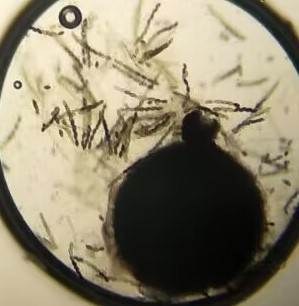
\includegraphics[height=0.3\textwidth]{img/perithecium}
        \label{fig:3-1}
    }
    \subfloat[子囊]{
        \centering
        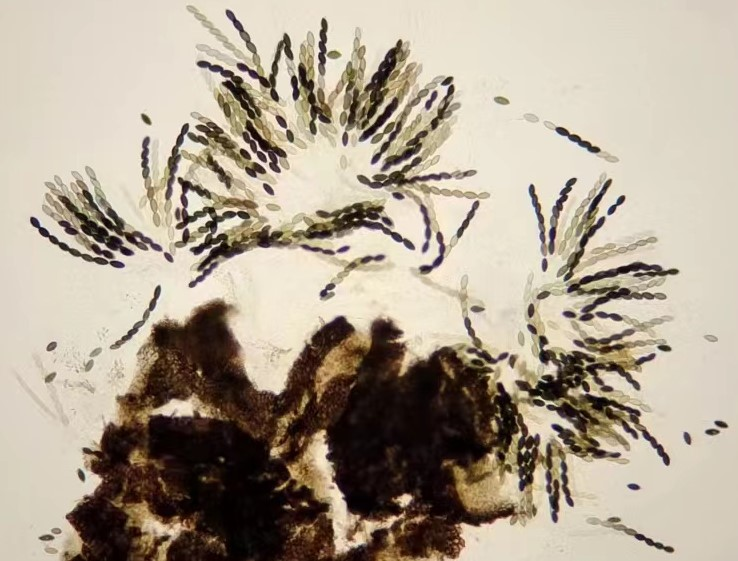
\includegraphics[height=0.3\textwidth]{img/ascus}
        \label{fig:3-2}
    }
    \label{fig:3}
    \caption{粗糙链孢霉的子囊果和子囊}
\end{figure}

\chapter{实验结果与分析}
\section{实验结果}
\begin{longtable}{cccccc}
    \hline
    \multirow{2}{*}{子囊类型} & \multirow{2}{*}{子囊孢子排列方式} & \multicolumn{3}{c}{各组员观察数} & \multirow{2}{*}{合计数} \\
    \cmidrule{3-5}
    & & 李泽华 & 余振洋 & 禹晓轩 & \\
    \hline
    \thead{第一次分裂分离 \\ (非交换型)} & \thead{$+ + + + - - - -$ \\ $- - - - + + + +$} & \thead{38 \\ 40} & \thead{46 \\ 37} & \thead{43 \\ 43} & 247\\
    \hline
    \thead{第二次分裂分离 \\ (交换型)} & \thead{$+ + - - + + - -$ \\ $- - + + - - + +$ \\ $+ + - - - - + +$ \\ $- - + + + + - -$} & \thead{7 \\ 2 \\ 3 \\ 2} & \thead{9 \\ 6 \\ 1 \\ 1} & \thead{6 \\ 4 \\ 2 \\ 4} & 47\\
    \hline
    \caption{本组数据统计}
\end{longtable}

除此以外, 我们还观察到了一些异常类型的子囊孢子, 如图\ref{fig:abnormal}

\begin{figure}[htbp]
    \centering

    \subfloat[4-4类型的异常孢子]{
        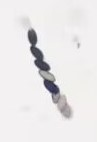
\includegraphics[height=0.4\textwidth]{img/abnormal}
        \label{fig:abnormal44}
    }
    \hfill
    \subfloat[2-6类型的异常孢子]{
        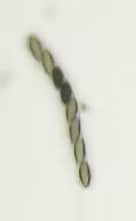
\includegraphics[height=0.4\textwidth]{img/abnormal26-1}
        \label{fig:abnormal26}
    }
    \hfill
    \subfloat[1-7类型的异常孢子]{
        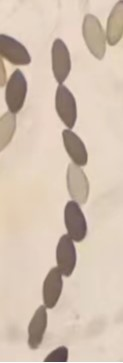
\includegraphics[height=0.4\textwidth]{img/abnormal17}
        \label{fig:abnormal17}
    }
    \caption{观察到的异常类型子囊孢子}
    \label{fig:abnormal}
\end{figure}

其中图\ref{fig:abnormal44}为$+++-+---$, 结合遗传学实验教材\upcite{2018LZUgeneticexp}, 我们认为这种异常类型的子囊孢子是由于子囊孢子的形成过程中, 减数分裂之后进行有丝分裂时, 纺锤体的重叠造成第4和第5孢子的位置互换导致的.
而图\ref{fig:abnormal26}($--++----$)和图\ref{fig:abnormal17}($+++-++++$)则是由于基因转换(gene conversion)\upcite{geneconver1, geneconver2, geneconver3}导致的.

\section{数据分析}
\subsection{计算重组率}
根据公式(\ref{eq:1}), 我们可以计算出各类子囊孢子的重组率,并进行可视化(如图\ref{fig:python}), 
得到的重组率为$7.993\%$

\begin{figure}[htbp]
    \centering
    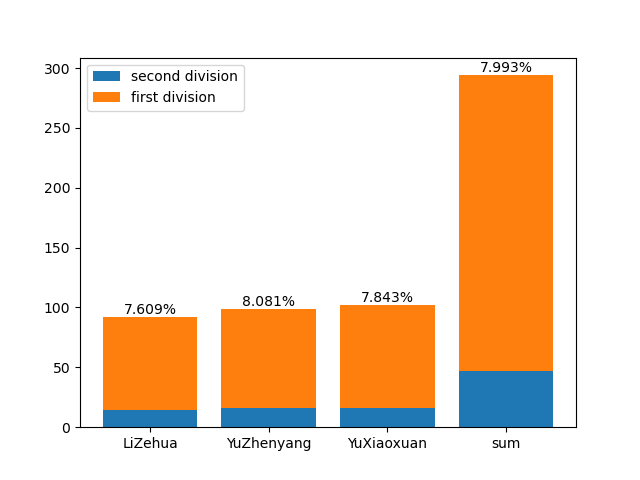
\includegraphics[width=0.8\textwidth]{img/python_result}
    \caption{重组率}
    \label{fig:python}
\end{figure}



\subsection{计算基因与着丝粒的距离}

将结果中的重组率换算为图距单位, 得到最终基因与着丝粒的距离为$7.993cM$.

\chapter{讨论}

本研究通过对粗糙链孢霉的遗传特性进行深入分析,采用顺序四分子的遗传学分析方法,旨在揭示粗糙链孢霉基因的分离和连锁交换规律。通过实验得到的结果和数据分析,为后续的遗传学研究提供了有益的参考。

在实验结果中,我们观察到了两种主要的子囊类型,分别是第一次分裂分离(非交换型)和第二次分裂分离(交换型)。通过对各组员的观察数据统计,我们得到了不同类型子囊孢子的数量,并计算了重组率。同时,我们还发现了一些异常类型的子囊孢子,这些异常类型的产生对于理解遗传现象提供了额外的信息。

通过数据分析,我们计算得到了重组率为7.993\%,并将其换算为基因与着丝粒的距离,得到约为7.993 cM。这个结果与预期值14.8cM有一定的偏差,这可能是由于实验过程中的技术差异, 环境因素等造成的。我们认为实验地兰州的海拔较高, 氧气含量较低, 可能会影响到粗糙链孢霉的生长, 从而影响到实验结果。

在实验过程中,我们还注意到了一些异常类型的子囊孢子,其中一些是由于有丝分裂过程中的纺锤体重叠引起的位置互换,另一些则是由基因转换导致的。这些异常类型的观察为研究粗糙链孢霉的遗传变异提供了有趣的现象,也为进一步深入了解其遗传机制提供了新的方向。

总体而言,本研究在深入理解粗糙链孢霉遗传学特性的基础上,通过实验得到了详实的结果,并通过数据分析得出了有意义的结论。这些结果为后续的遗传学研究提供了重要的参考,也为更深入地探讨粗糙链孢霉的遗传机制和基因功能奠定了基础。

%论文后部
\backmatter


%=======%
%引入参考文献文件
%=======%
\bibdatabase{bib/database}%bib文件名称 仅修改bib/ 后部分
\printbib
%\nocite{*} %显示数据库中有的,但是正文没有引用的文献



\Appendix
点击打开\href{https://github.com/zehua0417/GeneticExperimentReport}{附录链接}


%\Thanks


%\Grade %这一句才是成绩页,上面是填写


\end{document}
